% !TeX spellcheck = es_ES
\documentclass[12pt, titlepage]{article}
\usepackage[letterpaper, margin=2.5cm]{geometry}
% MATEMATICAS
\usepackage{amsmath}
\usepackage{amsfonts}
\usepackage{amssymb}
\usepackage{physics}
% IDIOMA %
\usepackage[utf8]{inputenc}
\usepackage[spanish]{babel}
\usepackage{url}
% IMAGENES
\usepackage{graphicx} 
\usepackage{float}
% COLORES
\usepackage{color}
\definecolor{verde}{RGB}{34, 139, 34}
\definecolor{gray}{rgb}{0.5,0.5,0.5}
\definecolor{mauve}{RGB}{253,151,31}
\definecolor{deepred}{RGB}{249,38,114}
\definecolor{azul}{RGB}{0, 0, 255}
\definecolor{cadena}{RGB}{160, 32, 240}
% CODIGO %
\usepackage{listings}

\lstset{
    frame=tb,
    language=MATLAB,
    aboveskip=3mm,
    belowskip=3mm,
    showstringspaces=false,
    columns=flexible,
    numbers=left,
    stepnumber=1,
    basicstyle={\small\ttfamily},
    numberstyle=\tiny\color{gray},
    keywordstyle=\color{azul},
    commentstyle=\color{verde},
    stringstyle=\color{cadena},
    breaklines=true,
    breakatwhitespace=true,
    tabsize=2,
    morekeywords={cell, strcat, textscan, permute},
    emph={},
    emphstyle=\color{deepred}
}
%opening
\title{Reporte Perceptrón Multicapa (MLP)}
\author{Barrera Pérez Carlos Tonatihu \\Boleta: 2016630023\\ Profesor: Moreno 
Armendariz Marco Antonio \\ Redes Neuronales \\ Grupo: 3CM2 }

\begin{document}

\maketitle
\tableofcontents
\newpage

\section{Introducción}
El objetivo del siguiente trabajo es sentar las bases de los principales puntos 
en el estudio del Perceptrón Multicapa (Multilayer Perceptron) entre los que 
están sus características, las partes que lo conforman y el como estas partes 
trabajan juntas para lograr el funcionamiento que el MLP presenta. Conociendo 
su funcionamiento se puede determinar cuales son las principales actividades en 
las que es empleada esta arquitectura de redes neuronales lo cual, a su vez, 
explica el porque dicha red es de tal importancia en el campo de las redes 
neuronales.
\\\\
Sin embargo, todo este conocimiento teórico seria nada si no se ve aplicado a 
algún problema en especifico, es debido a esto que en esta práctica se empleo 
el perceptrón multicapa para realizar la aproximación de señales (la cual es 
una de las principales aplicaciones que tiene esta red) esta aproximación fue 
desarrollada utilizando la herramienta MATLAB, entre las principales 
características que tiene el programa desarrollado están.
\begin{itemize}
 \item Entrada de datos por parte del usuario.
 \item Distintos métodos para determinar la convergencia de la red.
 \item Graficación de los resultados obtenidos por el perceptrón.
\end{itemize}
Aunado a esta implementación se encuentra la discusión de resultados en la cual 
se realiza un análisis de los datos obtenidos de los resultados 
experimentales con distintos casos de pruebas. Al hacer dicho análisis se llego 
a diferentes conclusiones respecto a la implementación realizada y en generar a 
la red neuronal utilizada como es el caso de sus ventajas y las limitaciones 
que tiene el uso de esta.
\newpage
\section{Marco teórico}
Además de presentar la teoría relacionada con el MLP es necesario explicar lo que es el algoritmo de propagación hacia atrás (o Backpropagation en inglés) que es la base del aprendizaje de esta arquitectura.

El perceptrón multicapa (Multilayer Perceptron) surge de la necesidad de tratar problemas que no son linealmente separables es por esto que Frank Rosenblatt y Bernard Widrow propusieron redes multicapa pero no pudieron generalizar los algoritmos necesarios para entrenar dichas redes.

Dicho algoritmo fue descrito hasta 1974 por Paul Werbos pero fue hasta 1980 cuando se empezó a divulgar y fue entonces cuando el MLP entrenado por el algoritmo de backpropagation se ha convertido en la red neuronal más utilizado. \cite{libro1}
\subsection{Perceptron multicapa}
Un perceptron multicapa es aquello en el cual la salida de una capa es la entrada de la siguiente capa, un ejemplo de esto es el mostrado en la figura \ref{fig:MLP} donde se presenta un MLP de tres capas. En un MLP cada capa puede tener diferente número de neuronas y distintas funciones de transferencia. Para poder diferenciar cada capa se utiliza un superindice como por ejemplo:
\[ \begin{bmatrix} R & S^1 & S^2 & S^3 & \dots & S^N \end{bmatrix} \]

\begin{figure}[H]
    \begin{center}
        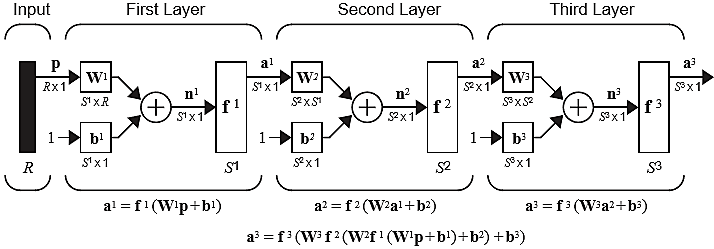
\includegraphics[width=16cm]{img/MLP.png}
        \caption{Perceptron de tres capas. \cite{libro1}}
        \label{fig:MLP}
    \end{center}
\end{figure}

En donde $S^1$ indica el número de neuronas de la capa uno, $S^2$ el número de neuronas en la capa dos y así consecutivamente. Esta misma estructura permite identificar la arquitectura de la red neuronal donde $R$ es el número de entradas. Para identificar el conjunto de funciones que se utiliza en cada capa se utiliza.

\[ \begin{bmatrix} F^1 & F^2 & F^3 & \dots & F^N \end{bmatrix} \]


Cada uno de estos elementos hace referencia alguna función de activación, las funciones que más se suelen utilizar son no lineales algunas de estas son.

\begin{itemize}
    \item Log-Sigmoid
    \[ a = \dfrac{1}{1+e^{-n}}\]
    \item Hyperbolic Tangent Sigmoid
    \[ a = \dfrac{e^n - e^{-n}}{e^n + e^{-n}}\]
    \item Linear
    \[ a = n\]
\end{itemize}

\begin{figure}[H]
    \begin{center}
        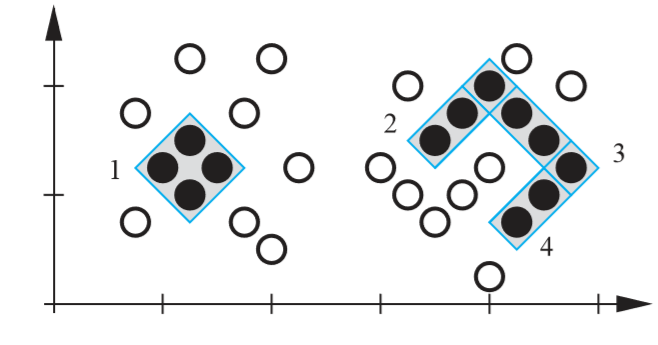
\includegraphics[width=7cm]{img/patrones.png}
        \caption{Clasificación de patrones. \cite{libro1}}
        \label{fig:clasificacion}
    \end{center}
\end{figure}

Las principales aplicaciones del MLP son:
\begin{itemize}
    \item Clasificación de patrones, objetos y caracteres como en la figura \ref{fig:clasificacion}.
    \item Aproximación de funciones.
    \item Compresión y codificación de información
    \item Reconocimiento de palabras (véase figura \ref{fig:palabras}).
    \item Segmentación de imágenes \cite{pdf}.
\end{itemize}

\begin{figure}[H]
    \begin{center}
        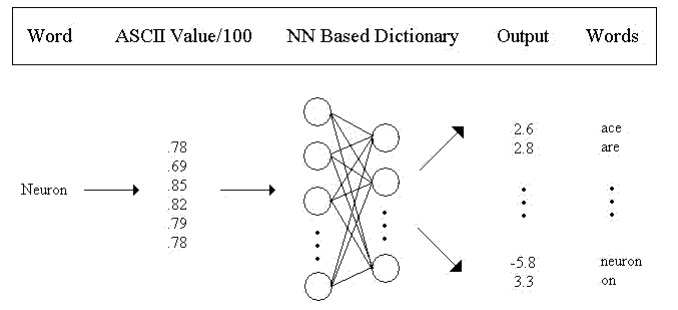
\includegraphics[width=12cm]{img/palabras.png}
        \caption{Diagrama del reconocimiento de palabras. \cite{pdf}}
        \label{fig:palabras}
    \end{center}
\end{figure}

La aproximación de señales se usa en sistemas de control en donde se trata de encontrar una función que pueda mapear mediciones de salidas a controles de entrada. Se puede realizar la aproximación de cualquier función si se tienen suficientes neuronas en las capas ocultas. 
\subsection{Backpropagation}
Para el estudio de backpropagation es importante conocer las ecuaciones que se usan en el aprendizaje que realiza. La primera de ellas está relacionada con las salidas de cada capa del MLP, estas ecuaciones son otra forma de representar la arquitectura de la figura \ref{fig:MLP}.

\begin{equation} \label{eq:1}
\boldsymbol{a}^0 = \boldsymbol{p}
\end{equation}
\begin{equation} \label{eq:2}
\boldsymbol{a}^{m+1} = \boldsymbol{f}^{m+1}(\boldsymbol{W}^{m+1}\boldsymbol{a}^{m}+\boldsymbol{b}^{m+1}
), \quad \text{Para $m=0, 1, \ldots M-1$}
\end{equation}
\begin{equation} \label{eq:3}
    \boldsymbol{a} = \boldsymbol{a}^{M}
\end{equation}
El valor de $M$ es el número de capas que tiene la red. La ecuación \ref{eq:1} hace referencia a que la capa uno tiene como entrada el conjunto de datos $\boldsymbol{p}$. Por otro lado la ecuación \ref{eq:3} es considerado como la salida final de la red neuronal.

El algoritmo backpropagation es una generalización del algoritmo LMS ya que ambos utilizan el error cuadrático medio, además utiliza un conjunto de entrenamiento compuesto por la entrada a la red y su correspondiente salida objetivo.
\[ \left\lbrace \boldsymbol{p_1}, \boldsymbol{t_1} \right\rbrace, \left\lbrace \boldsymbol{p_2}, \boldsymbol{t_2} \right\rbrace, \dots, \left\lbrace \boldsymbol{p_Q}, \boldsymbol{t_Q} \right\rbrace  \]
El objetivo de utilizar el una entrada y un target es utilizar un algoritmo de aprendizaje y con ello minimizar el error de salida de la red, dicho error es calculado con la siguiente formula.
\[ F(\boldsymbol{x}) = E \left[ \boldsymbol{e}^{T}\boldsymbol{e} \right] = E \left[ (\boldsymbol{t-a})^{T}(\boldsymbol{t-a}) \right]  \]
Aquí, $\boldsymbol{x}$ es el vector de pesos y bias de la red. Para una iteración (la propagación de un dato) esta ecuación se convierte en.
\[ \hat{F} (\boldsymbol{x}) = E \left[ \boldsymbol{e}^{T}\boldsymbol{e} \right] = E \left[ (\boldsymbol{t-a})^{T}(\boldsymbol{t-a}) \right]  \]
Esto hace que el algoritmo de gradiente descendente para pesos y bias sea.
\begin{equation} \label{eq:4}
w_{i, j}^{m}(k+1) = w_{i, j}^{m}(k) - \alpha \frac{\partial \hat{F}}{\partial w_{i, j}^{m}}
\end{equation}

\begin{equation} \label{eq:5}
b_{i}^{m}(k+1) = b_{i}^{m}(k) - \alpha \frac{\partial \hat{F}}{\partial b_{i}^{m}}
\end{equation}

Para poder trabajar con estas ecuaciones se debe de utilizar la regla de la cadena para facilitar el calculo de las derivadas parciales. Esto produce que se definan nuevos elementos los cuales son las sensitividades de $\hat{F}$ para cada elemento en cada capa de la red, dichas sensitividades producen los siguientes cambios.
\begin{equation} \label{eq:6}
\frac{\partial \hat{F}}{\partial w_{i, j}^{m}} = s_{i}^{m}a_{j}^{m-1}
\end{equation}
\begin{equation} \label{eq:7}
\frac{\partial \hat{F}}{\partial b_{i}^{m}} = s_{i}^{m}
\end{equation}
Al remplazar \ref{eq:6} y \ref{eq:7} en las ecuaciones \ref{eq:4} y \ref{eq:5} respectivamente y generalizando dichas ecuaciones a toda la matriz de pesos y bias para cada capa obtenemos las siguientes expresiones.

\begin{equation} \label{eq:8}
\boldsymbol{W}^{m}(k+1) = \boldsymbol{W}^{m}(k) - \alpha \boldsymbol{s}^{m} (\boldsymbol{a}^{m-1})^T
\end{equation}

\begin{equation} \label{eq:9}
\boldsymbol{b}^{m}(k+1) = \boldsymbol{b}^{m}(k) - \alpha \boldsymbol{s}^{m}
\end{equation}
Ahora lo importante es definir $\boldsymbol{s}^{m}$ para cada capa $\boldsymbol{m}$ de la red neuronal. Para la ultima capa del perceptrón, la capa $\boldsymbol{M}$ la sensitividad queda definida como:
\begin{equation} \label{eq:10}
    \boldsymbol{s^M} = 
    -2\boldsymbol{\dot{F}^{M}}(\boldsymbol{n^{M}})(\boldsymbol{t-a})
\end{equation}
Mientras que para el resto de las capas la sensitividad es:
\begin{align*}
\boldsymbol{s}^M &= 
-2\boldsymbol{\dot{F}}^{M}(\boldsymbol{n}^{M})(\boldsymbol{t-a}) \\
\boldsymbol{s}^{m} &= 
\boldsymbol{\dot{F}}^{m}(\boldsymbol{n}^{m})(\boldsymbol{W}^{m+1})^{T}
\boldsymbol{s}^{m+1} & & \text{para $m=M-1, \ldots, 2, 1$} \\
\text{donde} \\
\boldsymbol{\dot{F}}^{m}(\boldsymbol{n}^{m}) &=
\begin{bmatrix}
\dot{f}^{m}(n_{1}^{m}) & 0 & \ldots & 0 \\
0 & \dot{f}^{m}(n_{2}^{m}) & \ldots & 0 \\
\vdots & \vdots & \ddots & \vdots \\
0 & 0 & \ldots & \dot{f}^{m}(n_{s^{m}}^{m})
\end{bmatrix} \\
\dot{f}^{m}(n_{j}^{m}) &= 
\frac{\partial \dot{f}^{m}(n_{j}^{m})}{\partial n_{j}^{m}}
\end{align*}
Finalmente la actualización de pesos y bias en cada iteración queda definido por las siguientes ecuaciones
\begin{align*}
\boldsymbol{W}^{m}(k+1) &= \boldsymbol{W}^{m}(k)-\alpha 
\boldsymbol{s}^{m}(\boldsymbol{a}^{m-1})^{T}, \\
\boldsymbol{b}^{m}(k+1) &= \boldsymbol{b}^{m}(k) - \alpha \boldsymbol{s}^{m}
\end{align*}
\newpage
\section{Resultados experimentales}
Se realizaron 3 experimentos para comprobar el funcionamiento del perceptrón multicapa, para cada experimento se introdujeron valores diferentes para cada parámetro de la arquitectura, esto debido a que cada función a aproximar necesita parámetros personalizados para su correcto funcionamiento.

Algunas constantes que se mantienen en todos los experimentos son que la entrada de datos y objetivos se realizan mediante archivos de texto, además para cada experimento se muestra la evolución del error de iteración de entrenamiento y de validación en estas gráficas se puede observar que el error de validación tiende a ser más alto que el error de entrenamiento.

También, se gráfica la evolución de pesos y bias para cada capa de la red neuronal, finalmente se muestra una comparación entre un conjunto de prueba y la salida que proporciona el MLP. Además de imprimir los valores finales de error de iteración, error de validación y error de prueba. Finalmente los valores finales de pesos y bias son almacenados en un archivo de texto, uno por cada capa de la red.
\subsection{Experimento 1}
Se trabajo con un conjunto de datos con 101 datos los cuales al graficar dan como resultado la figura \ref{fig:original1}.

Los valores que se ingresaron son los que se muestran en la figura \ref{fig:entrada1} los valores más importantes que se tienen aquí son el factor de aprendizaje $\alpha=0.03$ el máximo numero de iteraciones a realizar el cual fue $iteraciones_{max} = 5000$ junto a un error permitido de $E_{it} = 0.005$ mientras que cada $200$ iteraciones se hará una iteración de validación con un máximo de tres incrementos consecutivos.
\begin{figure}[H]
    \begin{center}
        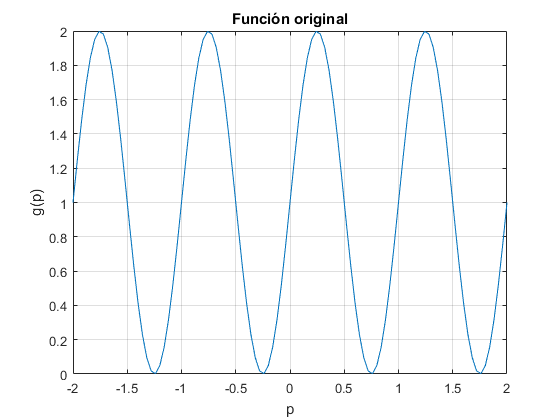
\includegraphics[width=10cm]{1/original.png}
        \caption{Función a aproximar en el experimento 1.}
        \label{fig:original1}
    \end{center}
\end{figure}
Para realizar las iteraciones de entrenamiento, prueba y validación la división del conjunto de datos fue $80-10-10$ respectivamente. Por otro lado, la arquitectura fue la siguiente.
\[ \left[ 1 \quad 6 \quad 1 \right] \]
\[ \left[ 3 \quad 1 \right] \]
donde
\begin{itemize}
    \item $3$ hace referencia a la función $tansig$.
    \item $1$ es la función $purelin$.
\end{itemize}
Una representación gráfica de esta arquitectura es la que se muestra en la figura \ref{fig:arqui1}. Los valores de pesos y bias de cada capa son inicializados entre $-1$ y $1$.
\begin{figure}[H]
    \begin{center}
        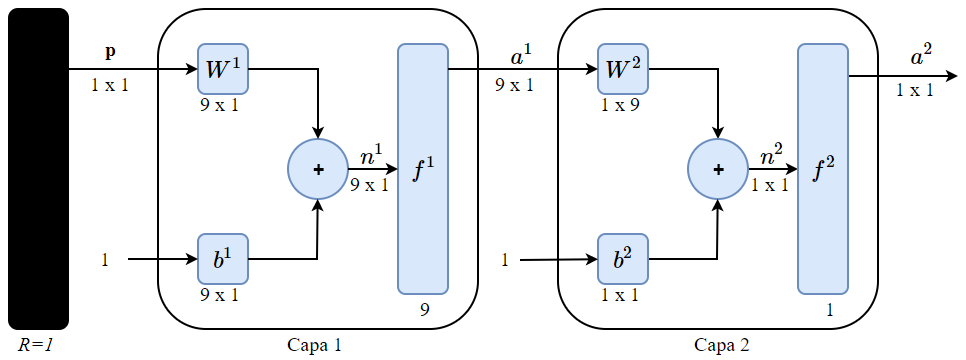
\includegraphics[width=14cm]{img/arqui1.png}
        \caption{Arquitectura del primer experimento.}
        \label{fig:arqui1}
    \end{center}
\end{figure}
Como se puede observar la primera capa tiene seis neuronas mientras que la segunda sólo tiene 1. Además las ecuaciones para la propagación hacia adelante y backpropagation se convierten en las siguientes.
\begin{figure}[H]
    \begin{align*}
        \boldsymbol{a}^0 &= \boldsymbol{p} \\
        \boldsymbol{a}^{1} &= logsig(\boldsymbol{W}^{1}\boldsymbol{a}^{0}+\boldsymbol{b}^{1}
        ) \\
        \boldsymbol{a}^{2} &= purelin(\boldsymbol{W}^{2}\boldsymbol{a}^{1}+\boldsymbol{b}^{2}
        ) \\
        \boldsymbol{a} &= \boldsymbol{a}^{2}
    \end{align*}
    \caption{Ecuaciones de propagación hacia adelante.}
\end{figure}
\begin{figure}[H]
    \begin{center}
        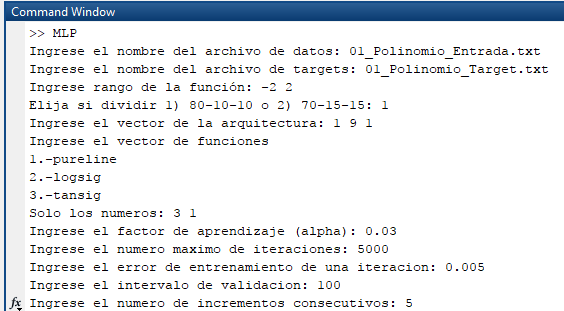
\includegraphics[width=14cm]{1/entrada.png}
        \caption{Entrada de datos del experimento 1.}
        \label{fig:entrada1}
    \end{center}
\end{figure}

\begin{figure}[H]
    \begin{align*}
    \boldsymbol{W}^{1}(k+1) &= \boldsymbol{W}^{1}(k) - \alpha \boldsymbol{s}^{1} (\boldsymbol{a}^{0})^T \\
    \boldsymbol{b}^{1}(k+1) &= \boldsymbol{b}^{1}(k) - \alpha \boldsymbol{s}^{1} \\
    \boldsymbol{W}^{2}(k+1) &= \boldsymbol{W}^{2}(k) - \alpha \boldsymbol{s}^{2} (\boldsymbol{a}^{1})^T \\
    \boldsymbol{b}^{2}(k+1) &= \boldsymbol{b}^{2}(k) - \alpha \boldsymbol{s}^{2} \\
    \boldsymbol{s}^2 &= 
    -2 \left[ 1 \right] (\boldsymbol{t-a}) \\
    \boldsymbol{s}^{1} &= 
    \boldsymbol{\dot{F}}^{1}(\boldsymbol{n}^{1})(\boldsymbol{W}^{2})^{T}
    \boldsymbol{s}^{2} \\
    \text{donde:} \\
    \boldsymbol{\dot{F}}^{1}(\boldsymbol{n}^{1}) &=
    \begin{bmatrix}
        1-(a_{1}^1)^2 & 0 & 0 & 0 & 0 & 0 \\
        0 & 1-(a_{2}^1)^2 & 0 & 0 & 0 & 0 \\
        0 & 0 & 1-(a_{3}^1)^2 & 0 & 0 & 0 \\
        0 & 0 & 0 & 1-(a_{4}^1)^2 & 0 & 0 \\
        0 & 0 & 0 & 0 & 1-(a_{5}^1)^2 & 0 \\
        0 & 0 & 0 & 0 & 0 & 1-(a_{6}^1)^2 \\
    \end{bmatrix}
    \end{align*}
    \caption{Ecuaciones del aprendizaje de la arquitectura de la figura \ref{fig:arqui1}.}
\end{figure}

\begin{figure}[H]
    \begin{center}
        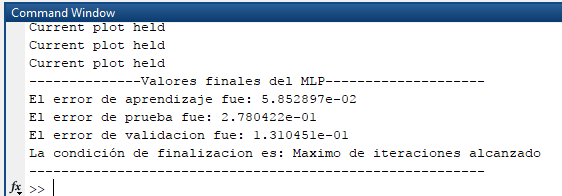
\includegraphics[width=14cm]{1/salida.png}
        \caption{Errores de cada iteración del experimento 1.}
        \label{fig:salida1}
    \end{center}
\end{figure}
Los errores finales se pueden observar en la figura \ref{fig:salida1}, además de que la condición de finalización fue que se alcanzo el número máximo de iteraciones.

Las siguientes imágenes son la evolución de pesos y bias de cada capa. Cada gráfica tiene comportamientos diferentes pero algo en lo que se parecen es que en algún punto de la gráfica ya no se producen tantas modificaciones en los valores que presentan.
\begin{figure}[H]
    \begin{center}
        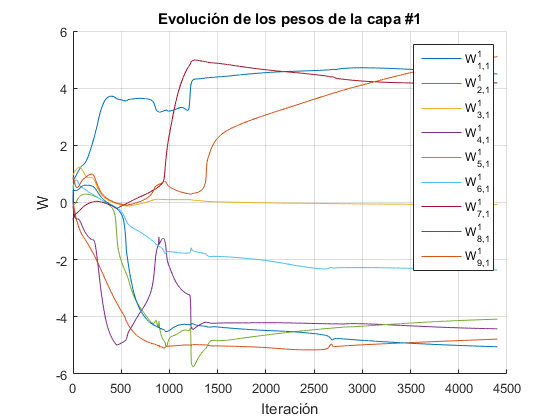
\includegraphics[width=12cm]{1/pesos1.png}
        \caption{Evolución de los pesos de la capa 1 del experimento 1.}
        \label{fig:pesos1}
    \end{center}
\end{figure}

\begin{figure}[H]
    \begin{center}
        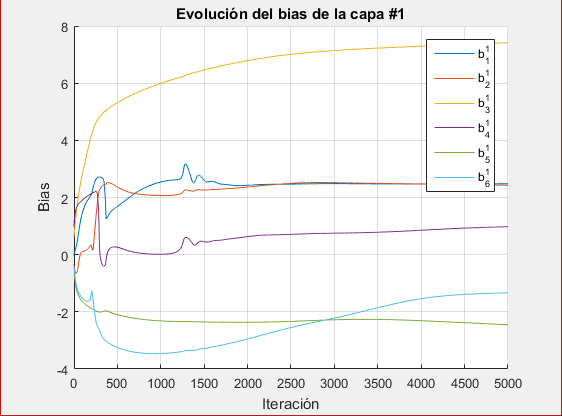
\includegraphics[width=12cm]{1/bias1.png}
        \caption{Evolución de los bias de la capa 1 del experimento 1.}
        \label{fig:bias1}
    \end{center}
\end{figure}

\begin{figure}[H]
    \begin{center}
        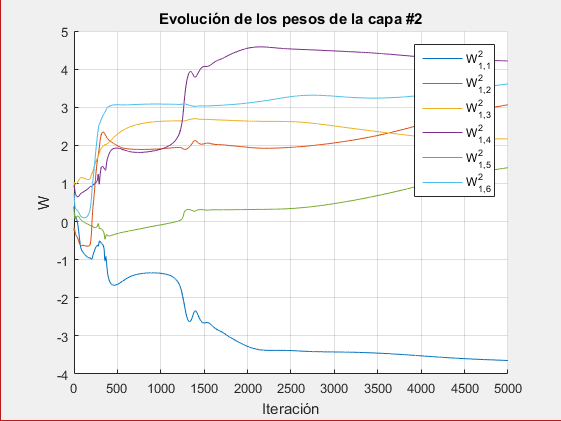
\includegraphics[width=12cm]{1/pesos2.png}
        \caption{Evolución de los pesos de la capa 2.}
        \label{fig:pesos2}
    \end{center}
\end{figure}

\begin{figure}[H]
    \begin{center}
        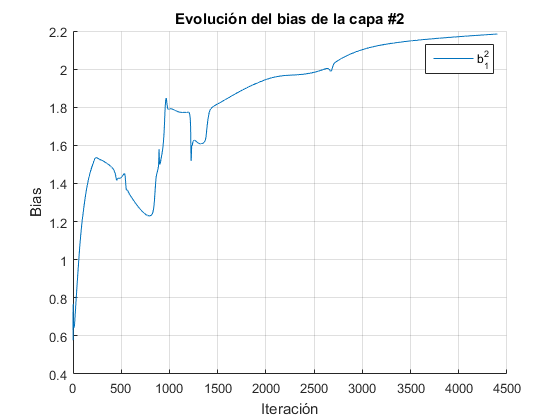
\includegraphics[width=12cm]{1/bias2.png}
        \caption{Evolución de los bias de la capa 2.}
        \label{fig:bias2}
    \end{center}
\end{figure}
Debido a que la división de los datos de entrada fue $80-10-10$ sólo se tienen $10$ datos que propagar se producen demasiados picos, por otro lado la aproximación se realiza casi completamente.
\begin{figure}[H]
    \begin{center}
        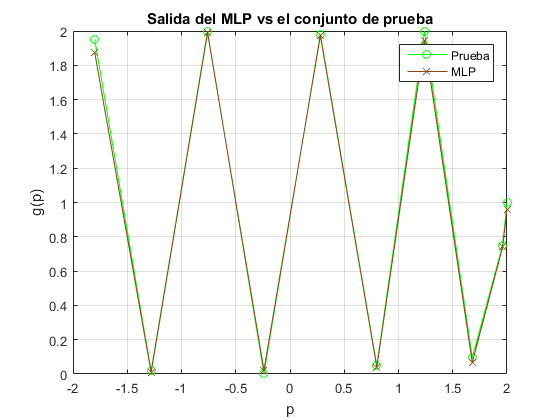
\includegraphics[width=12cm]{1/prueba.png}
        \caption{Comparación de las gráficas}
        \label{fig:prueba1}
    \end{center}
\end{figure}
Se puede observar que el error llega un punto en el que disminuye de una manera muy lenta hasta el final de todas las iteraciones.
\begin{figure}[H]
    \begin{center}
        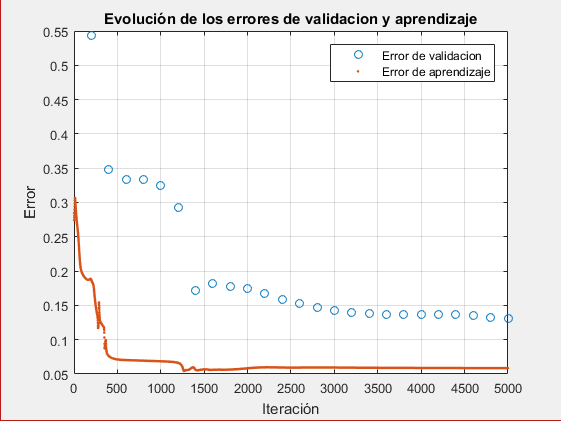
\includegraphics[width=16cm]{1/error.png}
        \caption{Evolución de los errores del experimento 1.}
        \label{fig:error1}
    \end{center}
\end{figure}
\newpage

\subsection{Experimento 2}
Para este experimento se trato con 241 datos los cuales al graficar dan como resultado la figura \ref{fig:original2}.

Los valores que se ingresaron son los que se muestran en la figura \ref{fig:entrada2} los valores más importantes que se tienen aquí son el factor de aprendizaje $\alpha=0.01$ el máximo numero de iteraciones a realizar el cual fue $iteraciones_{max} = 5000$ junto a un error permitido de $E_{it} = 0.0005$ mientras que cada $100$ iteraciones se hará una iteración de validación con un máximo de tres incrementos consecutivos.
\begin{figure}[H]
    \begin{center}
        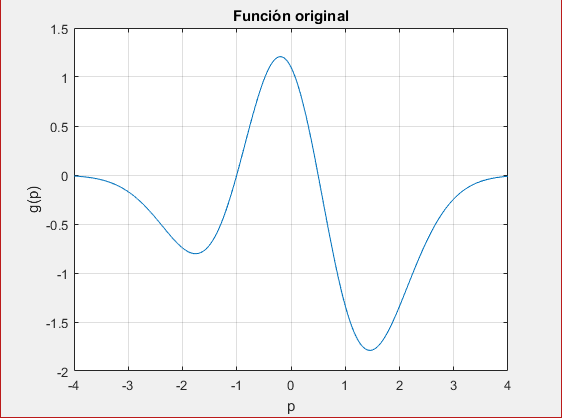
\includegraphics[width=12cm]{2/original.png}
        \caption{Función a aproximar en el experimento 2.}
        \label{fig:original2}
    \end{center}
\end{figure}
En esta ocasión la división de los datos fue $70-15-15$ para conjunto de entrenamiento, prueba y validación respectivamente. Por otro lado, la arquitectura fue la siguiente.
\[ \left[ 1 \quad 6 \quad 1 \right] \]
\[ \left[ 2 \quad 1 \right] \]
donde
\begin{itemize}
    \item $3$ hace referencia a la función $logsig$.
    \item $1$ es la función $purelin$.
\end{itemize}
Una representación gráfica de esta arquitectura es la que se muestra en la figura \ref{fig:arqui2}. Los valores de pesos y bias de cada capa son inicializados entre $-1$ y $1$.
\begin{figure}[H]
    \begin{center}
        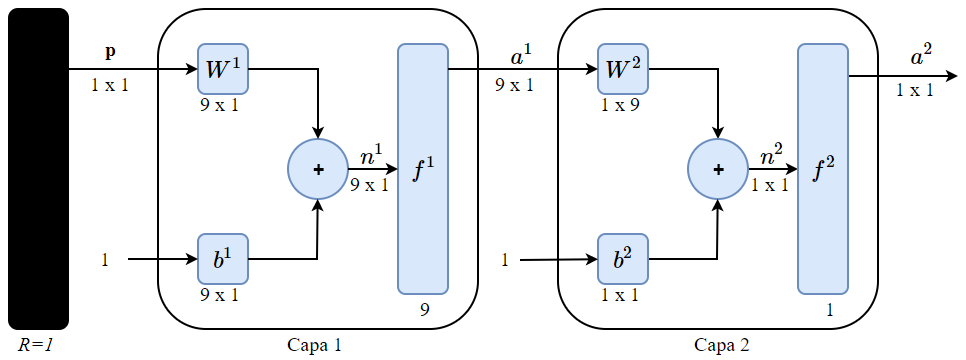
\includegraphics[width=14cm]{img/arqui1.png}
        \caption{Arquitectura del segundo experimento.}
        \label{fig:arqui2}
    \end{center}
\end{figure}
De nueva cuenta se tienen seis neuronas en la primera capa y sólo una en la segunda, lo cual genero las siguientes ecuaciones de propagación hacia adelante y backpropagation.

\begin{figure}[H]
    \begin{align*}
    \boldsymbol{a}^0 &= \boldsymbol{p} \\
    \boldsymbol{a}^{1} &= logsig(\boldsymbol{W}^{1}\boldsymbol{a}^{0}+\boldsymbol{b}^{1}
    ) \\
    \boldsymbol{a}^{2} &= purelin(\boldsymbol{W}^{2}\boldsymbol{a}^{1}+\boldsymbol{b}^{2}
    ) \\
    \boldsymbol{a} &= \boldsymbol{a}^{2}
    \end{align*}
    \caption{Ecuaciones de propagación hacia adelante.}
\end{figure}

\begin{figure}[H]
    \begin{center}
        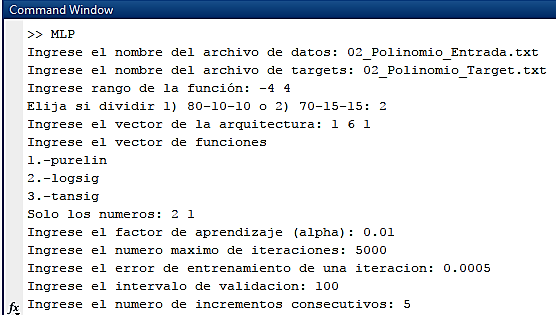
\includegraphics[width=14cm]{2/entrada.png}
        \caption{Entrada de datos del experimento 2.}
        \label{fig:entrada2}
    \end{center}
\end{figure}

\begin{figure}[H]
    \begin{align*}
    \boldsymbol{W}^{1}(k+1) &= \boldsymbol{W}^{1}(k) - \alpha \boldsymbol{s}^{1} (\boldsymbol{a}^{0})^T \\
    \boldsymbol{b}^{1}(k+1) &= \boldsymbol{b}^{1}(k) - \alpha \boldsymbol{s}^{1} \\
    \boldsymbol{W}^{2}(k+1) &= \boldsymbol{W}^{2}(k) - \alpha \boldsymbol{s}^{2} (\boldsymbol{a}^{1})^T \\
    \boldsymbol{b}^{2}(k+1) &= \boldsymbol{b}^{2}(k) - \alpha \boldsymbol{s}^{2} \\
    \boldsymbol{s}^2 &= 
    -2 \left[ 1 \right] (\boldsymbol{t-a}) \\
    \boldsymbol{s}^{1} &= 
    \boldsymbol{\dot{F}}^{1}(\boldsymbol{n}^{1})(\boldsymbol{W}^{2})^{T}
    \boldsymbol{s}^{2} \\
    \text{donde:} \\
    \boldsymbol{\dot{F}}^{1}(\boldsymbol{n}^{1}) &=
    \begin{bmatrix}
    (1-a_{1}^1)(a_{1}^1) & 0 & 0 & 0 & 0 & 0 \\
    0 & (1-a_{2}^1)(a_{2}^1) & 0 & 0 & 0 & 0 \\
    0 & 0 & (1-a_{3}^1)(a_{3}^1) & 0 & 0 & 0 \\
    0 & 0 & 0 & (1-a_{4}^1)(a_{4}^1) & 0 & 0 \\
    0 & 0 & 0 & 0 & (1-a_{5}^1)(a_{5}^1) & 0 \\
    0 & 0 & 0 & 0 & 0 & (1-a_{6}^1)(a_{6}^1) \\
    \end{bmatrix}
    \end{align*}
    \caption{Ecuaciones del aprendizaje de la arquitectura de la figura \ref{fig:arqui2}.}
\end{figure}

Los errores finales fueron, para el error de validación fue $2.61 x 10^{-3}$, para el de prueba fue $2.37x10^{-3}$ mientras que para el de aprendizaje fue $4.49x10^{-4}$ dichos valores se encuentran en la figura \ref{fig:salida2}, además de que la condición de finalización fue que el error de aprendizaje fue menor que el error de iteración.
\begin{figure}[H]
    \begin{center}
        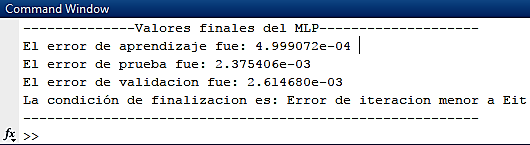
\includegraphics[width=14cm]{2/salida.png}
        \caption{Errores de cada iteración del experimento 2.}
        \label{fig:salida2}
    \end{center}
\end{figure}
Las siguientes imágenes son la evolución de pesos y bias de cada capa. Cada gráfica tiene comportamientos diferentes pero algo en lo que se parecen es que en algún punto de la gráfica ya no se producen tantas modificaciones en los valores que presentan.
\begin{figure}[H]
    \begin{center}
        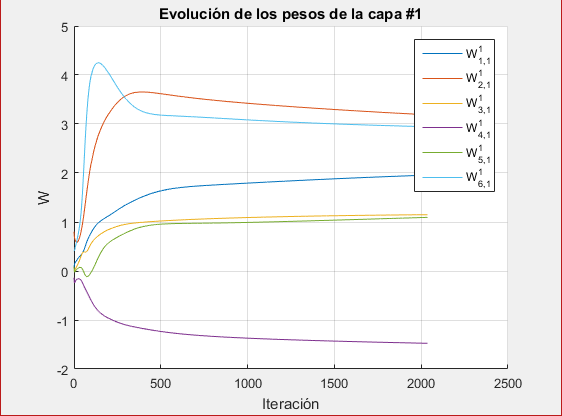
\includegraphics[width=13cm]{2/pesos1.png}
        \caption{Evolución de los pesos de la capa 1 del experimento 2.}
        \label{fig:pesos3}
    \end{center}
\end{figure}

\begin{figure}[H]
    \begin{center}
        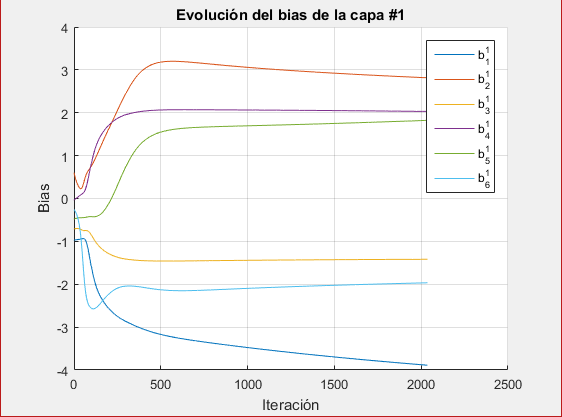
\includegraphics[width=13cm]{2/bias1.png}
        \caption{Evolución de los bias de la capa 1 del experimento 2.}
        \label{fig:bias3}
    \end{center}
\end{figure}

\begin{figure}[H]
    \begin{center}
        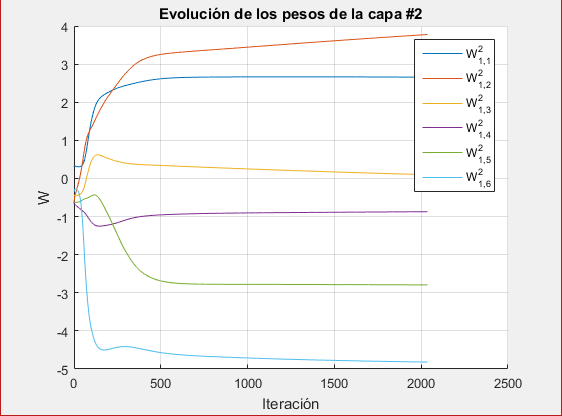
\includegraphics[width=13cm]{2/pesos2.png}
        \caption{Evolución de los pesos de la capa 2.}
        \label{fig:pesos4}
    \end{center}
\end{figure}

\begin{figure}[H]
    \begin{center}
        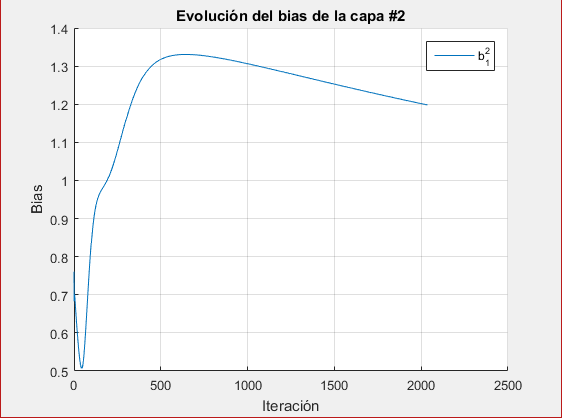
\includegraphics[width=13cm]{2/bias2.png}
        \caption{Evolución de los bias de la capa 2.}
        \label{fig:bias4}
    \end{center}
\end{figure}
Finalmente tenemos la comparación de la salida del MLP y los valores reales, ya que el error es muy bajo la aproximación se realiza en casi todos los puntos con excepción de los primeros valores de la gráfica
\begin{figure}[H]
    \begin{center}
        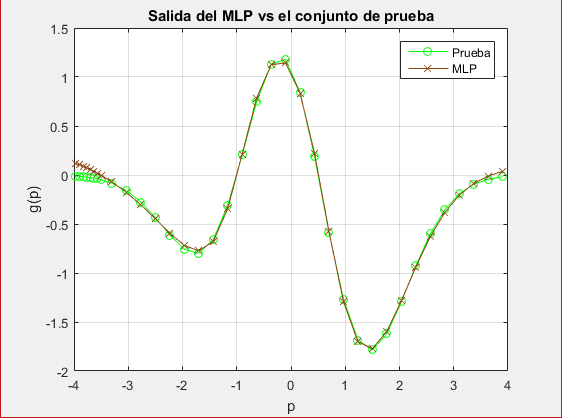
\includegraphics[width=16cm]{2/prueba.png}
        \caption{Comparación de las gráficas}
        \label{fig:prueba2}
    \end{center}
\end{figure}
El comportamiento de la gráfica anterior se puede ver reflejado en la evolución del error en el cual incluso el error de validación es más pequeño con cada iteración que se genera.
\begin{figure}[H]
    \begin{center}
        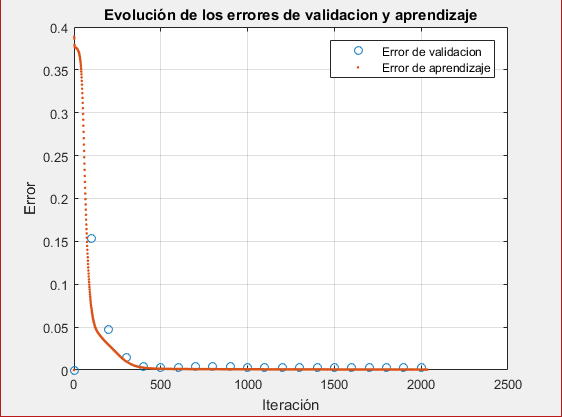
\includegraphics[width=16cm]{2/error.png}
        \caption{Evolución de los dos errores.}
        \label{fig:error2}
    \end{center}
\end{figure}

\newpage

\subsection{Experimento 3}
La cantidad de datos con los que se trabajo para este tercer experimento fueron 701 los cuales dan como resultado la gráfica que se muestra en la imagen \ref{fig:original3}.

Por otro lado, los parámetros que se utilizaron se encuentras en la figura \ref{fig:entrada3} es importante señalar los valores que juegan el papel más crucial en el funcionamiento del MLP los cuales son el factor de aprendizaje que fue$\alpha=0.005$, el máximo numero de iteraciones a realizar el cual fue $iteraciones_{max} = 5000$ y se tiene un error de iteración de $E_{it} = 0.0005$ además de tener este parámetro de finalización se debe realizar una iteración de validación cada $100$ iteraciones y si se detecta un incremento consecutivo tres veces se detendrá el aprendizaje para evitar el sobreentrenamiento.
\begin{figure}[H]
    \begin{center}
        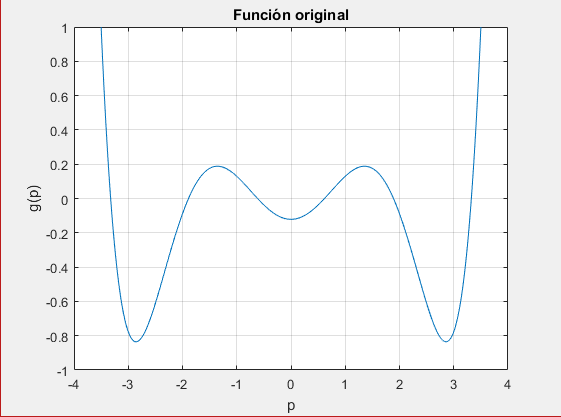
\includegraphics[width=14cm]{3/original.png}
        \caption{Función a aproximar en el experimento 3.}
        \label{fig:original3}
    \end{center}
\end{figure}
En esta ocasión la división de los datos fue $80-10-10$ para conjunto de entrenamiento, prueba y validación respectivamente. Por otro lado, la arquitectura fue la siguiente.
\[ \left[ 1 \quad 5 \quad 5 \quad 1 \right] \]
\[ \left[ 2 \quad 3 \quad 1 \right] \]
donde
\begin{itemize}
    \item $2$ hace referencia a la función $logsig$.
    \item $3$ hace referencia a la función $logsig$.
    \item $1$ es la función $purelin$.
\end{itemize}
Para que esta arquitectura sea más fácil de entender se presenta una representación gráfica de dicha arquitectura (véase figura \ref{fig:arqui3}). Al igual que en los experimentos anteriores los valores de pesos y bias son inicializados entre $-1$ y $1$.
\begin{figure}[H]
    \begin{center}
        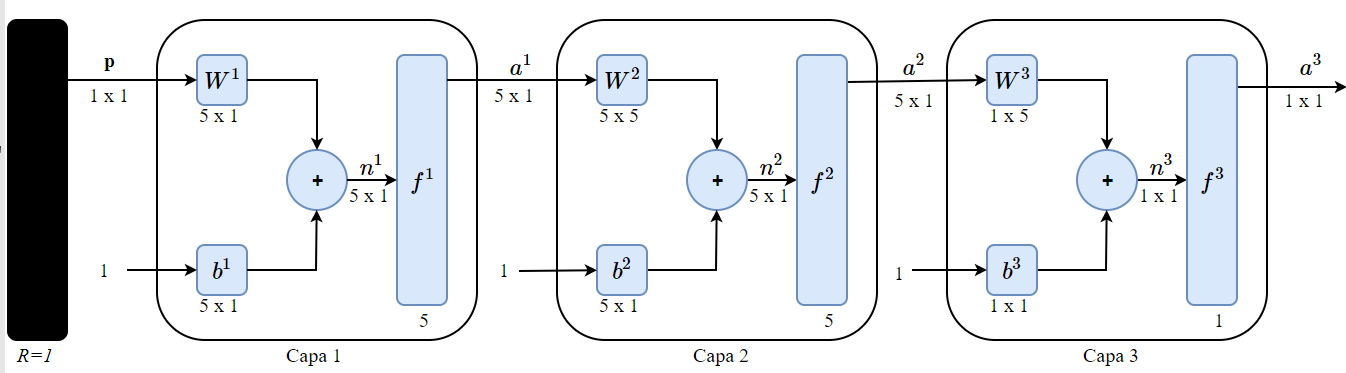
\includegraphics[width=16cm]{img/arqui3.png}
        \caption{Arquitectura del tercer experimento.}
        \label{fig:arqui3}
    \end{center}
\end{figure}
Como se puede observar, en este experimento no se tiene la misma arquitectura que en los experimentos anteriores ya que después de muchas pruebas se llego a la conclusión que esta arquitectura con 3 capas es la que mejor aproximo la función.
\begin{figure}[H]
    \begin{center}
        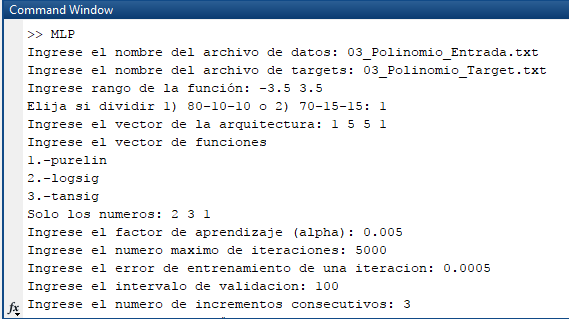
\includegraphics[width=14cm]{3/entrada.png}
        \caption{Entrada de datos del experimento 3.}
        \label{fig:entrada3}
    \end{center}
\end{figure}
En la figura \ref{fig:salida3} se puede observar que la condición de finalización fue que se alcanzo el máximo de iteraciones, por otro lado, el error de aprendizaje fue $5.08 x 10^{-3}$, el error de validación fue $6.606 x 10^{-2}$ y para el error de prueba fue $6.674 x 10^{-2}$.
\begin{figure}[H]
    \begin{center}
        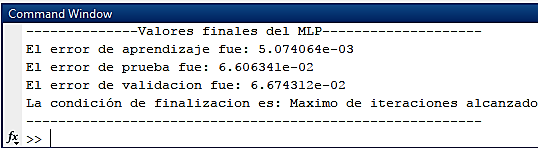
\includegraphics[width=14cm]{3/salida.png}
        \caption{Errores de cada iteración del experimento 3.}
        \label{fig:salida3}
    \end{center}
\end{figure}
Las siguientes imágenes son la evolución de pesos y bias de cada capa. Cada gráfica tiene comportamientos diferentes pero algo en lo que se parecen es que en algún punto de la gráfica ya no se producen tantas modificaciones en los valores que presentan.
\begin{figure}[H]
    \begin{center}
        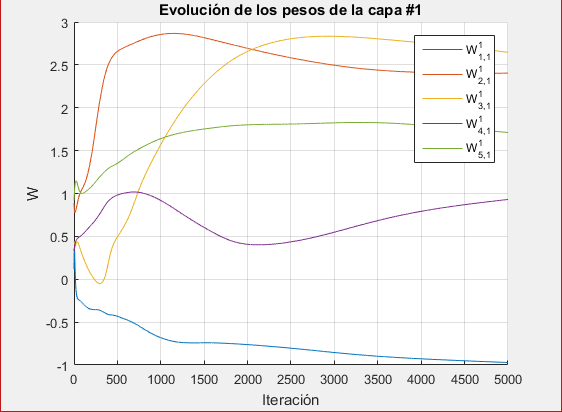
\includegraphics[width=12cm]{3/pesos1.png}
        \caption{Evolución de los pesos de la capa 1 del experimento 3.}
        \label{fig:pesos5}
    \end{center}
\end{figure}

\begin{figure}[H]
    \begin{center}
        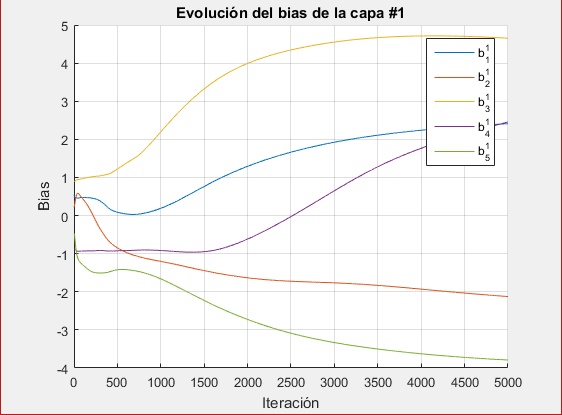
\includegraphics[width=12cm]{3/bias1.png}
        \caption{Evolución de los bias de la capa 1 del experimento 3.}
        \label{fig:bias5}
    \end{center}
\end{figure}

\begin{figure}[H]
    \begin{center}
        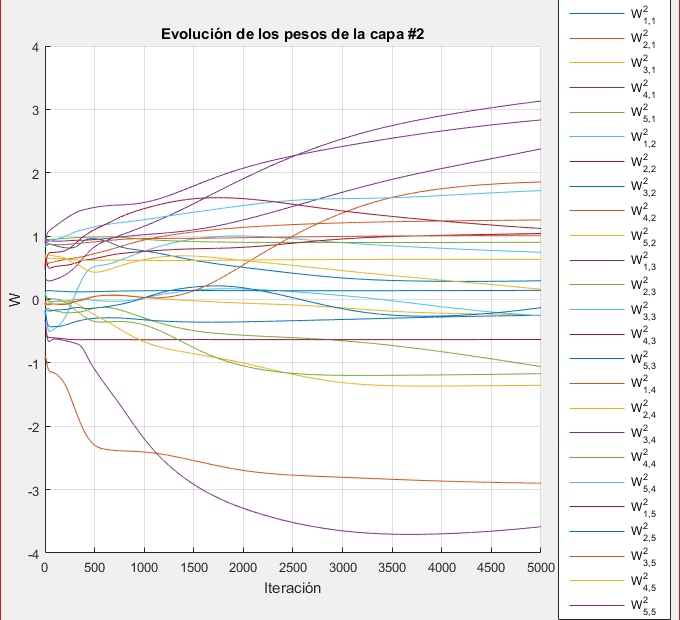
\includegraphics[width=16cm]{3/pesos2.png}
        \caption{Evolución de los pesos de la capa 2.}
        \label{fig:pesos6}
    \end{center}
\end{figure}

\begin{figure}[H]
    \begin{center}
        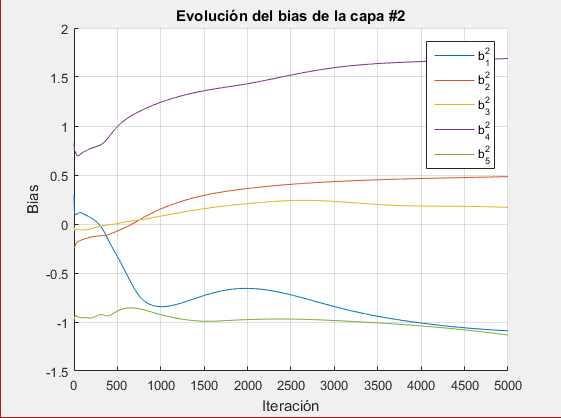
\includegraphics[width=12cm]{3/bias2.png}
        \caption{Evolución de los bias de la capa 2.}
        \label{fig:bias6}
    \end{center}
\end{figure}

\begin{figure}[H]
    \begin{center}
        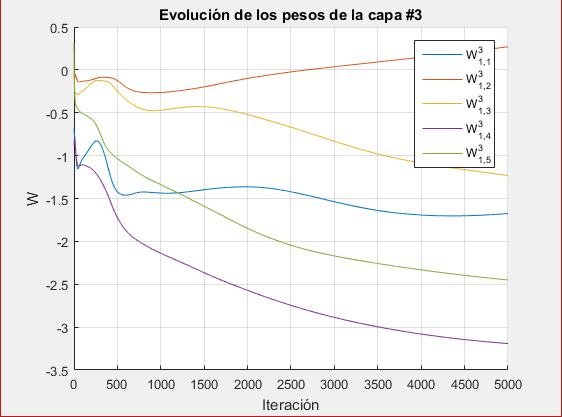
\includegraphics[width=12cm]{3/pesos3.png}
        \caption{Evolución de los pesos de la capa 3.}
        \label{fig:pesos7}
    \end{center}
\end{figure}

\begin{figure}[H]
    \begin{center}
        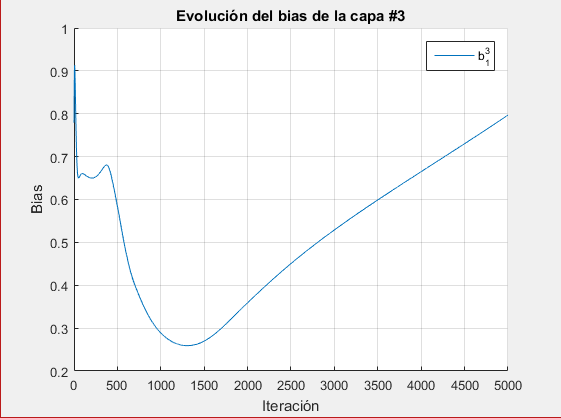
\includegraphics[width=12cm]{3/bias3.png}
        \caption{Evolución de los bias de la capa 3.}
        \label{fig:bias7}
    \end{center}
\end{figure}

Finalmente tenemos la comparación de la salida del MLP y los valores reales, ya que el error es muy bajo la aproximación se realiza en casi todos los puntos con gran precisión a excepción de los extremos de la función en los que hay cambios muy drásticos que no se modelan correctamente.
\begin{figure}[H]
    \begin{center}
        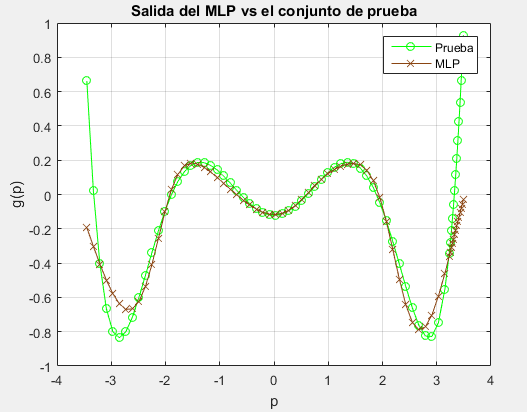
\includegraphics[width=12cm]{3/prueba.png}
        \caption{Comparación de las gráficas}
        \label{fig:prueba3}
    \end{center}
\end{figure}
El comportamiento de la función se puede ver reflejado en la evolución del error en el cual incluso el error de validación es más pequeño con cada iteración que se genera.
\begin{figure}[H]
    \begin{center}
        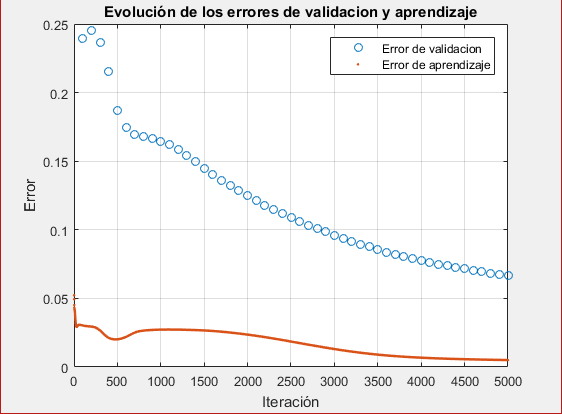
\includegraphics[width=14cm]{3/error.png}
        \caption{Evolución de los dos errores.}
        \label{fig:error3}
    \end{center}
\end{figure}

\newpage
\section{Discusión de resultados}
Después de realizar cada experimento se pueden sacar varias conclusiones respecto al comportamiento del perceptron multicapa y el porque ocurrió lo que se muestra en las gráficas además de que se puede hacer para mejorar los resultados proporcionados por el perceptron multicapa.

En el primer experimento debido a que se tenían pocos dados la aproximación falla en algunos puntos, aunado al hecho que dicha señal tiene demasiados máximos y mínimos hace que el comportamiento no sea regular, para poder tratar con los máximos y mínimos se pueden agregar más capas o neuronas lo cual aumentaría el numero de parámetros que se deben de ajustar, esto seria suficiente; pero debido a que la cantidad de datos que se tienen son pocos se produciría demasiado ruido, el cual se vería reflejado en una mejor aproximación en la forma general de la gráfica pero al mismo tiempo produciría muchas variaciones a lo largo de toda la función lo cual se conoce como sobreentrenamiento.

El experimento dos tuvo el mejor resultado de todas las pruebas realizadas, en este casi todos los puntos pudieron ser aproximados a excepción de los primeros valores, esto se pudo ser consecuencia de que no se realizo una distribución homogénea optima antes de iniciar el entrenamiento lo cual pudo provocar que no hubiera suficientes datos de entrenamiento al inicio del intervalo; pero a pesar de esto el entrenamiento fue tan bueno que no se necesito tener más iteraciones debido a que el error de aprendizaje fue bastante bajo. Es por esto que una posible mejora que se podría hacer para incrementar la precisión es establecer un error de aprendizaje más bajo para permitir un mayor numero de iteraciones, establecer los valores de pesos, bias y factor de aprendizaje en números que hagan que el entrenamiento sea más rápido.

Por otro lado, el tercer experimento ocurrió algo pelicular debido a que el error de aprendizaje fue bastante bajo lo cual se nota en la gráfica \ref{fig:error3}; pero al mismo tiempo no se aproximo correctamente en los extremos de la función, esto pudo ser causado por no tener suficientes datos en esas secciones de la gráfica o por el hecho de que los cambios fueron tan bruscos que no se hicieron correctamente las aproximaciones, este error no se pudo resolver aumentando el numero de neuronas o capas ya que generaba ruido en la aproximación y provocaba que el aprendizaje terminara por sobreentrenamiento. De tener una mejor selección de bias y de pesos al igual que factor de aprendizaje esto podría mejorar el entrenamiento esta conclusión surge del hecho de que en el experimento dos tanto el error de validación y aprendizaje son bastante bajos pero en este experimento el error de validación es mayor que el de aprendizaje.

Finalmente, el cuarto experimento es el menos satisfactorio de todos, se probaron diversas arquitecturas y configuraciones de estas pero ninguna pudo hacer que se produjera un resultado positivo, los cambios que se generaban en la aproximación y en la evolución del error son mínimos, esto debe de ser causa de que la función a aproximar es demasiado caótica (véase figura \ref{fig:original4}), al inicio de dicha función incluso pareciese que no es una función continua y que solo da saltos entre un valor y otro, sin duda esto merma la eficiencia del perceptrón multicapa.
\newpage
\section{Conclusiones}
Sin duda alguna el perceptrón multicapa es una herramienta sumamente poderosa no por nada es la arquitectura más utilizada actualmente, esta práctica solo es una muestra de ello debido a que solo se utilizo para la aproximación de funciones. Sin embargo, es importante tener en cuenta que para su correcto funcionamiento se deben considerar diversos factores.

Dichos factores afectaron a la elaboración de esta práctica como el hecho de no tener tantos datos como ocurrió en el primer experimento realizado. Otra cuestión que es importante mencionar es que el tiempo de ejecución puede llegar a ser bastante alto por lo que contar con un buen hardware es de suma importancia, en este caso los tiempos alcanzaron casi 10 minutos para la máxima cantidad de datos y 5000 iteraciones. Lo cual puede parecer poco tiempo pero si se tratara de usar en un ambiente real se puede llegar a trabajar con millones de datos por lo cual no seria de utilidad, dicho problema se podría solucionar al utilizar otro lenguaje de programación más rápido como es el caso de C.

Finalmente, es evidente que se puede mejorar el entrenamiento utilizando valores de pesos, bias y factor de aprendizaje más específicos por lo que seria de gran utilidad tener un pre procesamiento de los datos que genere mejores valores de dichos parámetros y no solo utilizar valores aleatorios.
\newpage
\bibliographystyle{apalike}
\bibliography{reporte}
\section{Anexo}
\begin{lstlisting}
function MLP()
    % Funcion principal del perceptron multicapa
    
    % Variables globales que se utilizan mucho y no cambian
    global FUNCIONES;
    global arqui;
    global vector_func;
    % Funciones que se pueden utilizar
    FUNCIONES = {@purelin, @logsig, @tansig};
    archivo_datos = input('Ingrese el nombre del archivo de datos: ', 's');
    archivo_targets = input('Ingrese el nombre del archivo de targets: ', 's');
    rango_entrada = input('Ingrese rango de la funcion: ', 's');
    entradas = load(archivo_datos);
    targets = load(archivo_targets);
    % Total de datos 
    num_datos = length(entradas);
    % Como se dividiran los datos
    division = input('Elija si dividir 1) 80-10-10 o 2) 70-15-15: ');
    divisor = .8;
    if division == 2
        divisor = .7;
    end
    % Total de datos de entrenamiento, prueba y validacion
    tam_entrenamiento = round(num_datos * divisor);
    tam_prueba = (num_datos - tam_entrenamiento) / 2;
    tam_validacion = tam_prueba;
    % Inicializacion de matrices
    datos_aprendizaje = zeros(tam_entrenamiento, 2);
    datos_validacion = zeros(tam_validacion, 2);
    datos_prueba = zeros(tam_prueba, 3);
    j = 1;
    k = 1;
    l = 1;
    i = 1;
    % Distribucion de los datos
    auxiliar = round(num_datos / (num_datos - tam_entrenamiento));
    tomar = 0;
    contador = 0;
    algo = 1;
    aux_aprendizaje = 0;
    while (i <= num_datos)
        if tomar == 1
            datos_prueba(j, 1) = entradas(i);
            datos_prueba(j, 2) = targets(i);
            j = j + 1;
            tomar = 0;
        elseif tomar == 2
            datos_validacion(k, 1) = entradas(i);
            datos_validacion(k, 2) = targets(i);
            k = k + 1;
            tomar = 0;
        else
            if aux_aprendizaje < tam_entrenamiento
                datos_aprendizaje(l, 1) = entradas(i);
                datos_aprendizaje(l, 2) = targets(i);
                l = l + 1;
                contador = contador + 1;
                aux_aprendizaje = aux_aprendizaje+1;
            else
                contador = auxiliar;
                i = i-1;
            end
            if contador == auxiliar
                contador = 0;
                if algo == 1
                    tomar = 1;
                    algo = 2;
                else
                    tomar = 2;
                    algo = 1;
                end
            end
        end
        i = i + 1;
    end
    arqui_entrada = input('Ingrese el vector de la arquitectura: ', 's');
    arqui_entrada = textscan(arqui_entrada, '%d', 'Delimiter', ' ' );
    arqui = permute(arqui_entrada{1}, [2, 1]);
    fprintf('Ingrese el vector de funciones\n');
    fprintf('1.-purelin\n2.-logsig\n3.-tansig\n')
    funciones_entrada = input('Solo los numeros: ', 's');
    funciones_entrada = textscan(funciones_entrada, '%d', 'Delimiter', ' ' );
    vector_func = permute(funciones_entrada{1}, [2, 1]);
    alpha = input('Ingrese el factor de aprendizaje (alpha): ');
    itmax = input('Ingrese el numero maximo de iteraciones: ');
    Eit = input('Ingrese el error de entrenamiento de una iteracion: ');
    itval = input('Ingrese el intervalo de validacion: ');
    num_val = input('Ingrese el numero de incrementos consecutivos: ');
    
    % Inicializacion de variables
    [W, b] = inicializar();
    incrementos = 0; % Contador incrementos
    Eval = 0; % Error de validacion
    error_aprendizaje = 0;
    % Archivo para almacenar el error de aprendizaje y validacion
    f_errores = fopen('errores.txt', 'w');
    % Variable para saber el criterio de finalizacion
    condicion_finalizacion = 0;
    % Comenzamos las iteraciones
    for iteracion = 1:itmax
        % Iteracion de valicacion
        if mod(iteracion, itval) == 0
            fprintf('Iteracion de validacion #%d: %d incre %d\n', iteracion, error_aprendizaje, incrementos);
            error_validacion = iteracion_validacion(W, b, datos_validacion);
            fprintf(f_errores, '%.10f 0\n', error_validacion);
            % Comparacion de errores de validacion
            if error_validacion > Eval
                incrementos = incrementos + 1;
            else
                incrementos = 0;
            end
            Eval = error_validacion;
            % Si alcanzamos el maximo de intecrementos terminamos
            if incrementos == num_val
                condicion_finalizacion = 1;
                break;
            end
        else
            % Iteracion aprendizaje
            [error_aprendizaje, W, b] = iteracion_aprendizaje(W, b, datos_aprendizaje, alpha);
            fprintf(f_errores, '%.10f 1\n', error_aprendizaje);
            % Si cumple la condicion terminamos
            if error_aprendizaje < Eit
                condicion_finalizacion = 2;
                break
            end
        end 
    end
    fclose(f_errores);
    % Realizar la iteracion de prueba
    [datos_prueba, Ep]= iteracion_prueba(W, b, datos_prueba);
    % Graficacion e impresion de resultados
    graficar_original(entradas, targets);
    graficar_errores(itmax, itval);
    guardar_valores_finales(W, b);
    graficar_salida(datos_prueba);
    graficar_pesos();
    graficar_bias();
    mostrar_resultados(error_aprendizaje, Ep, Eval, condicion_finalizacion);
end

function graficar_original(entradas, targets)
    % Graficamos la funcion original
    figure('Name', 'Funcion original');
    plot(entradas, targets);
    hold;
    grid;
    title('Funcion original');
    xlabel('p');
    ylabel('g(p)');
end

function graficar_salida(datos_prueba)
    % Grafica de comparacion de resultados
    figure('Name', 'Salida del MLP vs el conjunto de prueba');
    plot(datos_prueba(:, 1)', datos_prueba(:, 2)', '-o', 'Color', 'g');
    hold;
    plot(datos_prueba(:, 1)', datos_prueba(:, 3)', '-x', 'Color', [0.54 0.27 0.07]);
    grid;
    title('Salida del MLP vs el conjunto de prueba');
    xlabel('p');
    ylabel('g(p)');
    legend('Prueba', 'MLP');
end

function graficar_pesos()
    % Grafica de evolucion de pesos de cada capa
    global arqui;
    capas = length(arqui) - 1;
    % Graficacion por capa
    for i = 1:capas
        titulo = strcat('Evolucion de los pesos de la capa #', num2str(i));
        figure('Name', titulo);
        grid;
        hold;
        archivo_W = strcat('W_', num2str(i));
        archivo_W = strcat(archivo_W, '.txt');
        W_bias = load(archivo_W);
        filas = length(W_bias);
        etiquetas = cell(1, arqui(i)*arqui(i+1));
        k = 1;
        for j = 1:arqui(i)
            for l = 1:arqui(i+1)
                etiquetas{k} = ['W^{' num2str(i) '}_{' num2str(l) ',' num2str(j) '}'];
                k = k + 1;
            end
        end
        plot(0:filas-1, W_bias);
        title(titulo);
        xlabel('Iteracion');
        ylabel('W');
        legend(etiquetas);
    end
end

function graficar_bias()
    % Graficar evolucion del bias de cada capa
    global arqui;
    capas = length(arqui) - 1;
    % Bias de cada capa
    for i = 1:capas
        titulo = strcat('Evolucion del bias de la capa #', num2str(i));
        figure('Name', titulo);
        grid;
        hold;
        archivo_b = strcat('b_', num2str(i));
        archivo_b = strcat(archivo_b, '.txt');
        f_bias = load(archivo_b);
        [filas, columnas] = size(f_bias);
        etiquetas = cell(1, columnas);
        for j = 1:columnas
            etiquetas{j} = ['b^{' num2str(i) '}_' num2str(j)];
        end;
        plot(0:filas-1, f_bias);
        title(titulo);
        xlabel('Iteracion');
        ylabel('Bias');
        legend(etiquetas);
    end
end

function graficar_errores(itmax, itval)
    % Grafica de la evolucion del error de iteracion y validacion
    vector_errores = load('errores.txt');
    vector_validacion = zeros(2, itmax/itval);
    vector_aprendizaje = zeros(2, itmax-itmax/itval);
    j = 1;
    k = 1;
    for i = 1: length(vector_errores)
        if vector_errores(i, 2) == 0
            vector_validacion(2, j) = vector_errores(i, 1);
            vector_validacion(1, j) = i;
            j = j + 1;
        else
            vector_aprendizaje(2, k) = vector_errores(i, 1);
            vector_aprendizaje(1, k) = i;
            k = k + 1;
        end
    end
    figure('Name', 'Evolucion de los errores de validacion y aprendizaje');
    
    plot(vector_validacion(1,:), vector_validacion(2,:), 'o');
    hold;
    plot(vector_aprendizaje(1,:), vector_aprendizaje(2,:), '.');
    grid;
    xlabel('Iteracion');
    ylabel('Error');
    title('Evolucion de los errores de validacion y aprendizaje');
    legend('Error de validacion', 'Error de aprendizaje');
end

function mostrar_resultados(error_aprendizaje, Ep, Eval, condicion_fin)
    % Imprimir valores importantes de la red
    fprintf('--------------Valores finales del MLP--------------------\n');
    fprintf('El error de aprendizaje fue: %d \n', error_aprendizaje);
    fprintf('El error de prueba fue: %d \n', Ep);
    fprintf('El error de validacion fue: %d \n', Eval);
    fprintf('La condicion de finalizacion es: ');
    if condicion_fin == 0
        fprintf('Maximo de iteraciones alcanzado\n');
    elseif condicion_fin == 1
        fprintf('Early stopping\n');
    else
        fprintf('Error de iteracion menor a Eit\n');
    end
    fprintf('---------------------------------------------------------\n');
end

function guardar_valores_finales(W, b)
    % Guardar la actualizacion de pesos y bias
    capas = length(W);
    % Hay un para bias y pesos por cada capa
    for i = 1:capas
        archivo_W = strcat('W_final_', num2str(i));
        archivo_W = strcat(archivo_W, '.txt');
        archivo_b = strcat('b_final_', num2str(i));
        archivo_b = strcat(archivo_b, '.txt');
        f_pesos = fopen(archivo_W, 'w');
        f_bias = fopen(archivo_b, 'w');
        fprintf(f_pesos, '%.10f ', W{i});
        fprintf(f_pesos, '\n');
        fprintf(f_bias, '%.10f ', b{i});
        fprintf(f_bias, '\n');
        fclose(f_pesos);
        fclose(f_bias);
    end
end

function [W, b] = inicializar()
    global arqui;
    capas = length(arqui) - 1;
    b = cell([1 capas]);
    W = cell([1 capas]);
    % Inicializar y guardar los pesos y bias de cada capa
    for i = 1:capas
        archivo_W = strcat('W_', num2str(i));
        archivo_W = strcat(archivo_W, '.txt');
        archivo_b = strcat('b_', num2str(i));
        archivo_b = strcat(archivo_b, '.txt');
        f_pesos = fopen(archivo_W, 'w');
        f_bias = fopen(archivo_b, 'w');
        S = arqui(i+1);
        R = arqui(i);
        W{i} = -1 + (1-(-1)) * rand(S, R);
        fprintf(f_pesos, '%.10f ', W{i});
        fprintf(f_pesos, '\n');
        b{i} = -1 + (1-(-1)) * rand(S, 1);
        fprintf(f_bias, '%.10f ', b{i});
        fprintf(f_bias, '\n');
        fclose(f_bias);
        fclose(f_pesos);
    end
end

% Derivadas de las funciones que se utilizan
function valor = derivada_purelin(~)
    valor = 1;
end

function valor = derivada_logsig(a)
    valor = (1-a) * a;
end

function valor = derivada_tansig(a)
    valor = 1 - (a * a);
end

function [datos_prueba, error_prueba] = iteracion_prueba(W, b, datos_prueba)
    % Propagacion del conjunto de prueba
    global vector_func;
    global FUNCIONES;
    error_prueba = 0;
    % Ciclo de los datos
    for i = 1:length(datos_prueba)
        p = datos_prueba(i, 1);
        % Ciclo de las capas de la red
        for j = 1:length(vector_func)
            % Seleccion de la funcion a utilizar
            a = FUNCIONES{vector_func(j)}(W{j} * p + b{j});
            p = a;
        end
        e = datos_prueba(i, 2) - a;
        error_prueba = error_prueba + (e' * e);
        datos_prueba(i, 3) = a;
    end
    % Regresamos el error de prueba
    error_prueba = error_prueba / length(datos_prueba);    
end

function [error_aprendizaje, W, b] = iteracion_aprendizaje(W, b, datos, alpha)
    global FUNCIONES;
    global vector_func;
    global arqui;
    error_aprendizaje = 0;
    capas = length(arqui) - 1;
    a = cell([1 capas]);
    s = cell([1 capas]);
    % Iteracion sobre todos los datos
    for i = 1:length(datos)
        p = datos(i, 1);
        % Propagacion hacia adelante
        for j = 1:length(vector_func)
            a{j} = FUNCIONES{vector_func(j)}(W{j} * p + b{j});
            p = a{j};
        end
        e = datos(i, 2) - a{capas};
        error_aprendizaje = error_aprendizaje + (e' * e);
        % Aprendizaje realizado
        s{capas} = -2 * e;
        % Modificamos cada capa
        for k = capas-1:-1:1
            W{k+1} = W{k+1} - alpha * s{k+1} * a{k}';
            b{k+1} = b{k+1} - alpha * s{k+1};
            Fn = zeros(arqui(k+1));
            if vector_func(k) == 1
                % PURELING
                derivada = @derivada_purelin;
            elseif vector_func(k) == 2
                % LOGSIG
                derivada = @derivada_logsig;
            else
                % TANSIG
                derivada = @derivada_tansig;
            end
            for j = 1:arqui(k+1)
                Fn(j, j) = derivada(a{k}(j));
            end
            s{k} = Fn * W{k+1}' * s{k+1};
        end
        % Primera capa
        W{1} = W{1} - alpha * s{1} * datos(i, 1)';
        b{1} = b{1} - alpha * s{1};
    end
    % Escritura de los valores
    for i = 1:capas
        archivo_W = strcat('W_', num2str(i));
        archivo_W = strcat(archivo_W, '.txt');
        archivo_b = strcat('b_', num2str(i));
        archivo_b = strcat(archivo_b, '.txt');
        f_pesos = fopen(archivo_W, 'a');
        f_bias = fopen(archivo_b, 'a');
        fprintf(f_pesos, '%.10f ', W{i});
        fprintf(f_pesos, '\n');
        fprintf(f_bias, '%.10f ', b{i});
        fprintf(f_bias, '\n');
        fclose(f_bias);
        fclose(f_pesos);
    end
    % Se devuelve el error
    error_aprendizaje = error_aprendizaje / length(datos);
end

function error_iteracion = iteracion_validacion(W, b, datos)
    global FUNCIONES;
    global vector_func;
    global arqui;
    error_iteracion = 0;
    M = length(arqui) - 1;
    a = cell([1 M]);
    % Ciclo de propagacion de cada dato
    for i = 1:length(datos)
        p = datos(i, 1);
        % Propagacion atravez de las capas
        for j = 1:length(vector_func)
            % Seleccion de la funcion a utilizar
            % con base a su capa
            a{j} = FUNCIONES{vector_func(j)}(W{j} * p + b{j});
            p = a{j};
        end
        % Suma del error
        e = datos(i, 2) - a{M};
        error_iteracion = error_iteracion + (e' * e);
    end
    % Guardar los datos de esta iteracion aunque no se modificaron
    for i = 1:M
        archivo_W = strcat('W_', num2str(i));
        archivo_W = strcat(archivo_W, '.txt');
        archivo_b = strcat('b_', num2str(i));
        archivo_b = strcat(archivo_b, '.txt');
        f_pesos = fopen(archivo_W, 'a');
        f_bias = fopen(archivo_b, 'a');
        fprintf(f_pesos, '%.10f ', W{i});
        fprintf(f_pesos, '\n');
        fprintf(f_bias, '%.10f ', b{i});
        fprintf(f_bias, '\n');
        fclose(f_bias);
        fclose(f_pesos);
    end
    % Se devuelve el error de la validacion
    error_iteracion = error_iteracion/length(datos);
end
\end{lstlisting}
\end{document}
